\documentclass{standalone}
\usepackage{tikz}
\usetikzlibrary{arrows}
\usetikzlibrary{positioning}
\usetikzlibrary{graphs}
\begin{document}
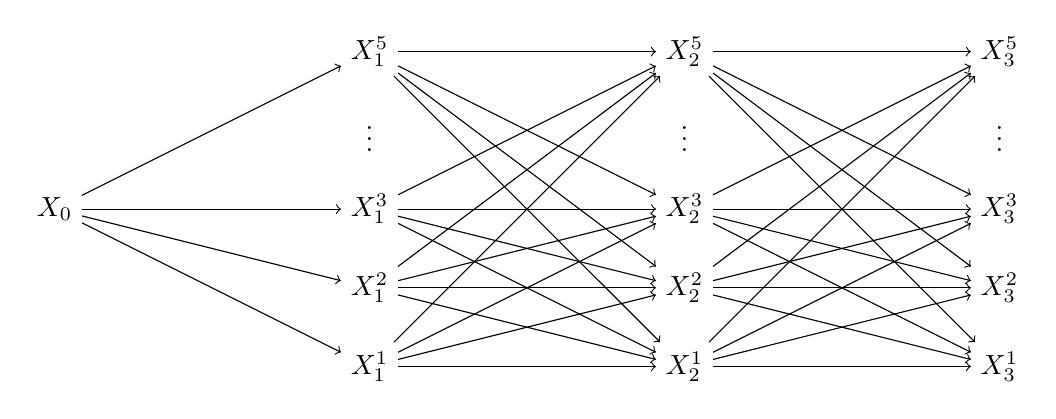
\begin{tikzpicture}
	\draw (0, 3) node[rectangle] (root) {$X_0$};
	
	\foreach \time in {1,2,3}{
		\foreach \x in {1,2,3,5}{
			\draw (4*\time, \x) node (\time\x) {$X_\time^\x$};
		}
		\draw (4*\time, 4) node (\time4) {$\vdots$};
	}
	\foreach \x in {1,2,3,5}{
			\draw[->] (root) -- (1\x);
	}

	\foreach \time in {1,2}{
		\foreach \x in {1,2,3,5}{
			\foreach \target in {1,2,3,5}
				\pgfmathtruncatemacro\nexttime{\time+1}
				\draw[->] (\time\x) -- (\nexttime\target);
		}
	}

\end{tikzpicture}
\end{document}